\chapter{Grundlagen}
Das PDF Dateiformat steht für Plattformunabhängigkeit, Hardwareunabhängigkeit, Konsistenz in Formatierung und Layout und soll ein möglichst originalgetreues Druckergebnis liefern. Der Leser soll ein PDF Dokument immer nach dem Prinzip \gls{wysiwyg} (What You See Is What You Get) in der Form betrachten und ausdrucken können wie es vom Ersteller des Dokuments festgelegt wurde.
\par
\begin{figure}[!htbp]
	\centering
	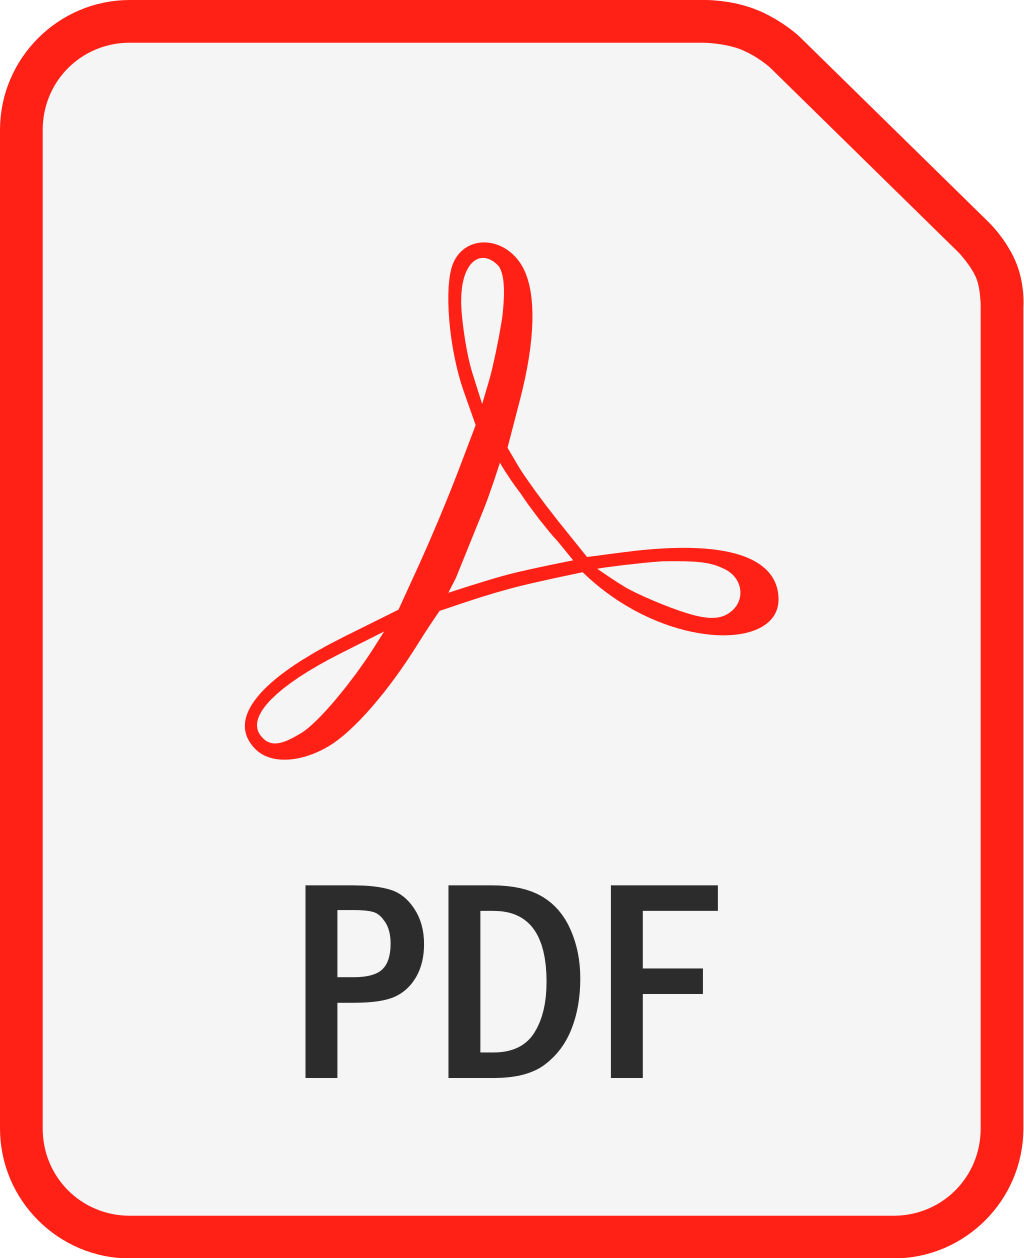
\includegraphics[scale=0.1]{"images/PDFfileIcon.png"}
	\caption{Adobe PDF Icon \cite{wiki-pdf-engl}}
	\label{fig:icon}
\end{figure}
PDF wurde im Jahr 1993 von dem 1982 gegründeten amerikanischen Softwareunternehmen Adobe Inc. veröffentlicht und ging aus dem 1991 von Adobe-Mitbegründer John Warnock gestarteten „Project Camelot" hervor\cite{wiki-pdf-de}. Ziel des Projekts war es, ein Dateiformat für elektronische Dokumente zu kreieren, sodass dieses Anwendungsprogramm, Betriebssystem und Hardware unabhängig sowie originalgetreu wiedergegeben werden kann. In Abbildung \ref{fig:icon} ist das Datei-Icon für PDF von Adobe zu sehen. \\
Anfangs war der Adobe Reader noch kostenpflichtig und PDF war für einen langen Zeitraum ein proprietäres Dateiformat, welches offengelegt im PDF Reference Manual von Adobe dokumentiert ist. Die Spezifikation von PDF ist seit 1993 kostenlos einsehbar \cite{wiki-pdf-engl}. Die \gls{iso} übernahm PDF im Jahr 2007 in den Standardisierungsprozess und seit der Veröffentlichung von PDF Version 1.7 am 1. Juli 2008 gilt PDF als Offener Standard als \gls{iso} 32000-1:2008\cite{wiki-pdf-de, wiki-pdf-engl}. Vorher war PDF ein proprietäres Dateiformat von Adobe. Der Begriff Offener Standard bezeichnet einen Standard, der für alle Teilhaber am Markt besonders leicht zugänglich, weiterentwickelbar und einsetzbar ist. Das bedeutet, dass der Standard von einer gemeinnützigen Organisation eingeführt, veröffentlicht sowie weiter bearbeitet wird und gleichmäßige Einflussnahme aller interessierten Parteien ermöglicht \cite{wiki-standard}. \\
Im gleichen Jahr publizierte Adobe eine Public Patent Licence zum \gls{iso} Standard 23000-1, also PDF Version 1.7, die royalty-free Rechte einräumt, um PDF-Implementierungen zu programmieren, verkaufen und verbreiten \cite{wiki-pdf-engl}. Royalty-free bedeutet hierbei, dass Computerherstellerfirmen pro verkauftes Endgerät keine Gebühren (royalties), sowie keine fixe Jahrespauschale bezahlen müssen \cite{wiki-roy-free}. Die letzte Dateiversion von PDF heißt PDF 2.0 und sie wurde im Jahr 2020 von der \gls{iso} standardisiert. Heute wird PDF seit 2006 von der PDF Association weiterentwickelt \cite{wiki-pdf-de}. 




\section{Wichtigste Features}
Die in den Unterkapiteln genannten Operationen auf dem PDF-Dateiformat beziehen sich hauptsächlich auf Adobe Acrobat-Werkzeuge. PDFs können Texte, Tabellen, Bilder, Pfade, Links, Buttons, Formulare, Audio-, Videoelemente und Funktionen enthalten. Rich Media-PDFs ermöglichen interaktive Inhalte, die eingebettet oder verlinkt werden können. Solche Elemente sind Bilder, Audio, Video oder Buttons, z.B. als digitaler Katalog \cite{wiki-pdf-engl}. Fonts und Bilder sollten grundsätzlich immer eingebettet werden. \\
In PDFs werden alle Informationen als nummerierte Objekte gespeichert. Objekte können zu Gruppen kombiniert werden. Der aktuelle Farbmodus im Dokument kann in andere Farbmodi konvertiert werden. Um die Navigation innerhalb eines PDF Dokuments zu erleichtern kann man anklickbare Inhaltsverzeichnisse und miniaturisierte Seitenvorschauen (Thumbnails) verwenden. Optional ist eine Gliederung als hierarchische Baumstruktur in Form von Lesezeichen möglich, mit der der Betrachter leichter durch das Dokument geführt werden kann. \\
PDF-Dateien enthalten grundsätzlich Metadaten. Bei Metadaten oder Metainformationen handelt es sich um strukturierte Daten, die sich auf Merkmale anderer Daten beziehen. Beispiele für Metadaten sind Name, Titel der Datei, Autor, Stichwörter zum Inhalt, das Datum der Speicherung. PDF-Dateien können Dateianhänge enthalten, die geöffnet und im lokalen Dateisystem abgespeichert werden können \cite{wiki-pdf-engl}. 

\subsection{WYSIWYG}
Ein PDF-Dokument hat ein festes Layout und eine feste Anzahl von Seiten. Unabhängig von der Software mit der das Dokument angezeigt wird oder mit welcher Hardware es ausgedruckt wird bleiben alle Elemente nach dem Prinzip \gls{wysiwyg} auf den Seiten immer exakt an derselben Position. Alle Layout- und Formatierungsangaben stammen aus der Erstellungsanwendung. Bei der Konvertierung von Dokumenten mit variablem Layout zu PDF, wie z.B. .txt-Dateien oder HTML muss der Inhalt auf die vorhandenen Seiten und den verfügbaren Platz verteilt werden. 

\subsection{Fonts}
Jedes Textzeichen ist ein abstraktes Symbol und ein Schriftzeichen beruht auf eine graphische Darstellung. Eine Schriftart ist in PDF als Objekt enthalten. Die Schriftart kann mit Werkzeugen in Acrobat bearbeitet werden. Der Text muss ausgewählt sein und es können darauf folgende Operationen angewandt werden: Farbveränderung in RGB, Transparenzen, Verschiebung, Löschen, Skalierung, Verzerrung bzw. Scherung, Spiegelung, Drehung, Beschneidung oder Ersetzung. Der RGB-Farbraum eignet sich lediglich für die Bildschirmdarstellung und beschreibt die für den Menschen 16,7 Millionen sichtbaren Farben mit Hilfe von additiver Farbmischung mittels Rot, Grün und Blau. Ein Farbraum umfasst die mathematischen Parameter als Daten für die Gesamtzahl der Farben, die auf einem Monitor, Druckmaterial, usw. darstellbar sind \cite{farbraum}. \\
In Adobe Acrobat Pro kann der gesamte Text pro Seite in Pfade konvertiert werden. Pfade sind mathematisch berechnete Linien, die aus gekrümmten Segmenten bestehen. Der Anfang und das Ende jedes Segments werden als Ankerpunkte bezeichnet und Pfade können geschlossen oder geöffnet sein. Die Form des Pfads kann durch die Griffpunkte an den Ankerpunkten modifiziert werden und Pfadsegmente können somit verformt werden \cite{adobe-pfade}.  Auf diese Weise kann man komplexe Formen für z.B. Firmenlogos oder auch eigene Schriftarten designen. Solche manuellen Pfade kann man vor allem in Adobes Illustrator, InDesign oder Photoshop erstellen. \\ 
PDF unterstützt Type-1-Fontformate, Multiple-Master-Fonts, TrueType-Fontformate, OpenType-Fontformate, Dfonts, \gls{cid} codierte Fonts und Composite-Fonts. Seit PDF 1.3 werden \gls{cid}-Schrifttypen als Abkömmlinge von Composite-Fonts unterstützt. \gls{cid} ist ein Synonym für das PostScript Type-0-Format, das eine Adressierung von mehr als 256 Zeichen ermöglicht und für Fonts mit einer großen Zeichenanzahl verwendet wurde \cite{typoinfo}. Composite-Fonts sind Basisschriften mit hierarchischem System. Die oberste hierarchische Ebene stellt den root font dar. Alle folgenden Fonts sind descendant fonts. Sie ermöglichten die Einführung von Type-1-Schriften im asiatischen Markt \cite{schneeberger}. Falls die Schriftart nicht im Dokument eingebettet wurde, wird sie aus der Ursprungsdatei möglicherweise durch eine Ersatzschrift des Benutzersystems im PDF-Programm substituiert \cite{schneeberger}. 

\subsection{Bilder}
Generell sollte für das Bearbeiten von Bildern ein externes Bildbearbeitungsprogramm verwendet werden, z.B. Photoshop oder das kostenlose Gimp. Dafür kann für die Bearbeitung in Photoshop das Bild mittels Acrobat Pro aus dem PDF extrahiert werden und später wieder im in Acrobat Pro geöffneten PDF ersetzt werden. Vektorgrafiken als Pfadobjekte und Rasterbilder als Pixelobjekte (Bitmap) können nach Auswahl verschoben, gelöscht, skaliert, verzerrt, gespiegelt, gedreht, die Deckkraft verändert, beschnitten oder ersetzt werden \cite{schneeberger}. Der Mehrgewinn an Vektorgrafiken liegt in dessen Eigenschaften, dass sie auflösungsunabhängig sind, da sie beliebig groß ohne Qualitätsverlust skaliert werden können und dass sie wesentlich weniger Speicherplatz benötigen als Rasterbilder. \\
Die Auflösung von Bildern kann in Acrobat neu berechnet werden. Niedrig aufgelöste Bilder behalten ihre Auflösung bei. Ein guter Neuberechnungsalgorithmus heißt bikubische Neuberechnung. Bei Schwarzweißbildern kann eine Neuberechnung zu unschönen Artefakten führen \cite{buehler}. Generell führt eine Neuberechnung der Auflösung in Bildbearbeitungsprogrammen zu besseren Ergebnissen als in Acrobat. Etwaige Pixelbearbeitungen wie Tonwertkorrekturen oder das Schärfen von Bildern können ausschließlich in Bildbearbeitungsprogrammen vorgenommen werden. 

\subsection{3D-Daten}
PDFs mit 3D-Inhalten bestehen aus dem U3D-Flächenmodell oder dem BREP/Flächenmodell PRC. Diese Flächenmodelle werden vorwiegend bei der Visualisierung von \gls{cad} Daten verwendet. Beide Formate können im Adobe Reader angezeigt, animiert, geschnitten und gemessen werden. Viele Drittanbieter PDF-Reader und die PDF-Viewer im Browser können eingebettete 3D-Daten meist nicht darstellen. Einige \gls{cad}-Programme ermöglichen einen 3D-PDF-Export oder Import \cite{wiki-pdf-de}. 

\subsection{Kommentare}
Ein Kommentarobjekt, das mit Dokumentenseiten verlinkt ist, besteht aus 2 technisch separaten Bausteinen. Zum einen werden Kommentare durch ein grafisches Element auf den zugehörigen Seiten symbolisiert, zum anderen wird der Kommentarinhalt in einem rechteckigen Kommentarbereich dargestellt. Ein Anwender kann die Darstellung des Kommentarobjekts je nach Geschmack modifizieren. Unüblicherweise kann ein Kommentar sogar als Video-Kommentar abgespielt werden. Die wichtigsten Kommentartypen sind Notizzettel, Textmarkierung, Stempel, Wasserzeichen, Textboxen, Formen, Freihand-Markierung, Audio, Video und 3D-Illustrationen. Kommentare können optional mit ausgedruckt werden \cite{softx}. 

\subsection{Verweise}
Technisch gesehen sind Verweise oder Hyperlinks spezialisierte Kommentare ohne Symboldarstellung. Auf der Seite wird ein Ausschnitt zur Platzierung des Verweises gewählt, der über einem Inhaltselement (Text oder Bild) liegt. Der Verweis zeigt auf eine Seite oder Seitenbereich im geöffneten Dokument, eine andere PDF-Datei, eine E-Mailadresse oder URL. Man kann sogar Zielobjekte mit einem im gesamten Dokument eindeutigen Namen einstellen \cite{softx}. 

\subsection{Formulare}
In PDFs kann man Formularfelder vom Typ Textfeld, Kontrollkästchen, Auswahlknopf, Kombinationsfeld, Auswahlliste, Schaltfläche, Barcode- oder Unterschriftsfeld erstellen. Ein Formularfeld ist ein Objekt zum befüllen und speichern von Felddaten. Die unterschiedlichen Formularfeldtypen weisen verschiedene Eigenschaften in Bezug auf Interaktivität und Gestaltung auf. Jedes Feld hat einen eindeutigen Namen im gesamten Dokument. Mit diesem unikalen Namen können Namensgruppen realisiert werden. Durch eine hierarchische Struktur mittels Teilnamen, die mit einem Punkt voneinander getrennt sind mit dem äußersten Gruppennamen zuerst geschrieben werden, können Felddaten noch besser und logischer beschrieben bzw. strukturiert werden. Jedes Feldobjekt geht Hand in Hand mit einem Widget, welches ein spezielles Kommentarobjekt zur Steuerung darstellt. Diese Widgets stehen für Werte oder Zustände der Felder und sind dafür verantwortlich, dass man Formulare im PDF-Dokument mit dem Computer, Tablet oder Smartphone ausfüllen kann. Außerdem ist es möglich unsichtbare Feldobjekte, die ohne das Widget platziert werden können, zu erstellen, um die PDF-Software anzusprechen. Häufiger werden mehrere Widgets mit einem Feldobjekt gekoppelt \cite{softx}. \\
Um elektronisch ausfüllbare Formulare zu verwenden müssen zusätzlich in Acrobat Formularfelder auf die entsprechenden Stellen platziert werden. Falls ein Listenfeld verwendet wird, sollte man eine Schrift für die Listeneinträge im PDF einbetten. Formulare können einen druckbaren und nicht druckbaren Teil enthalten. In der Druckvorstufe müssen vor dem Druck alle Formularfelder eliminiert werden, damit alle Schriften eingebettet werden können \cite{schneeberger}. Es gibt 2 verschiedene Möglichkeiten von PDF Formularen: AcroForms (Acrobat Forms) oder Adobes proprietäre \gls{xfa} forms, welche mit Version 2.0 von der \gls{iso} als veraltet markiert wurden. \gls{xfa}s Haupterweiterungen zu \gls{xml} sind rechnergestützte, aktive Tags und sein Datenformat ist kompatibel mit anderen Systemen, Anwendungen und Technologiestandards \cite{wiki-xfa}. \gls{xml} ist eine Sprache zur Markierung von Inhalten mit Hilfe von Tags, um die Struktur zu beschreiben und Elemente zu identifizieren \cite{schneeberger}. AcroForms unterstützen das Abschicken (submit), Zurücksetzen und Importieren von Daten. Die submit-Aktion transferiert die Namen und Werte eines ausgewählten interaktiven Formularfelds zu einer vordefinierten URL. In der Praxis werden Formulare in einem Grafik- oder Layoutprogramm gestaltet und als PDF exportiert.

\subsection{Incremental Update}
Die ursprüngliche Version einer PDF-Datei bleibt erhalten, während das incremental update die Änderungen im Dokument enthält. Professionelle PDF-Programme können ähnlich einer Versionsverwaltung jede geänderte Version des Dokuments laden. Bei einfacheren PDF-Programmen wird lediglich die letzte Version geladen. Bei Verwendung von incremental updates kann man digital unterschriebene Dokumente ändern ohne dass die Unterschrift ungültig wird, da die Dokumentversion mit der digitalen Unterschrift ein andere Version ist als die nachträgliche Änderung. Dabei muss die digitale Unterschrift als incremental update gespeichert werden, sonst würde sie bei nachträglicher Dokumentenmodifikation unabhängig von der Änderungsart verfallen. Folglich sollten mehrfach signierte Dokumente ebenfalls mit der Option incremental update gespeichert werden \cite{softx}. Pro incremental update steigt der Speicherbedarf einer PDF-Datei.

\subsection{Kompression}
PDF-Dateien sind komprimiert und haben üblicherweise einen Bruchteil der Größe des Ursprungsformats. Dies wird durch Vermeidung von Redundanzen, Erhöhung der Entropie (Zeichendichte) und Weglassen von Informationen bewerkstelligt. Im Allgemeinen gibt es verlustlose und verlustbehaftete Kompression. Die Kompressionsalgorithmen \gls{rle}, die genauso effiziente LZW, Flate-Komprimierung, ZIP und CCITT gehören zur verlustfreien Kompression. Zur verlustbehafteten Kompression zählen JPEG, JBIG2 und JPEG2000 \cite{schneeberger}.  Kompressionsalgorithmen sind nicht auf bestimmte Dateiformate beschränkt. In PDF können die folgenden Kompressionsalgorithmen für Bilder verwendet werden: IP, \gls{rle}, JPEG, JPEG2000, CCITT und JBIG2. Eine hohe Bildqualität im PDF bedeutet eine größere Datei. Faktoren, die die Bildqualität beeinflussen, sind Breite x Höhe des Bildes, Farbtiefe, Farbraum und die Kompressionsmethode \cite{softx}. \\
Außerdem ist es möglich eine Datenreduktion durch Neuberechnung zu erzielen. Hierbei wird das verlustbehaftete Downsampling verwendet und führt häufig zu nicht befriedigenden Ergebnissen. Es gibt als Neuberechnungsmethoden die eher im Ergebnis mangelhafte Kurzberechnung, sowie die besseren durchschnittliche und bikubische Neuberechnungen. Neuberechnungen in Photoshop führen generell zu besseren Ergebnissen als in Adobe Acrobat Distiller \cite{schneeberger}. \\
PDF-Dateien können zur Weboptimierung serialisiert (linearisiert) werden, sodass Teile des PDFs während des Ladevorgangs dargestellt werden. Liegen unkomprimierte Elemente im Dokument vor, werden diese beim Speichern durch die Flate-Komprimierung, die auch den ZIP-Algorithmus verwendet, komprimiert.

\subsection{Ebenen}
Ebenen werde auch als Optional Content Layers bezeichnet und stellen quasi mehrere Inhaltsschichten auf einer einzelnen PDF-Seite dar, wobei jede Seite im Dokument beliebig viele Ebenen enthalten kann. Jede Ebene kann PDF-Inhalt sozusagen logisch gruppieren und die Bearbeitung von Inhalten auf einer Ebene wirkt sich nur auf diese Ebene aus. Man kann Inhalte auch mehreren Ebenen zuordnen oder keiner Ebene. Ebenen können ein- und ausgeblendet, ihre Reihenfolge verändert, gesperrt, zusammengeführt, aus anderen PDF-Dateien importiert und für unterstützende Dateiformate von Adobeprogrammen, z.B. Photoshop, Illustrator oder InDesign, exportiert werden. Zusätzlich kann man eine Ebenennavigation mit Hilfe von Links und Lesezeichen konstruieren, um Ebenensichtbarkeit für den Betrachter zu steuern \cite{adobe-ebenen}. 

\subsection{Portfolio}
Ein Portfolio bezeichnet eine Datei bestehend aus anderen Dateien, die kein Hauptdokument enthält, sondern lediglich eine Pseudo-Seite. Diese Pseudo-Seite wird von Portfolio inkompatiblen PDF-Programmen angezeigt. Zusätzlich können andere PDF-Dateien und andere Dateiformate im PDF-Hauptdokument eingebettet werden \cite{softx}. 

\subsection{JavaScript}
In PDF kann man Ereignisse Aktionen zuordnen, d.h. bei Eintreffen eines Ereignisses wird automatisch eine Aktion ausgeführt. Ein Ereignis ist eine bestimmte Statusänderung von Objekten oder ein interaktives Anwenderereignis. Dabei kann man als Aktion JavaScript-Code aufrufen, dessen Aktion mit Lesezeichen, Verweisen, Seiten und Dokumentereignissen verknüpft ist. Auf Formularfeldern kann ebenfalls JavaScript angewandt werden \cite{softx}. Diese JavaScript-Erweiterung für Acrobat ist eine proprietäre Technologie von Adobe. Viele andere nicht-Adobe PDF-Programme bieten keine Unterstützung für JavaScript \cite{wiki-pdf-engl}. 
\section{PDF Dateiformate}
PDF hat zahlreiche Dateiformate, von denen die meisten standardisiert wurden, hervorgebracht. Jedes Dateiformat ist einem individuellen Anwendungsbereich zugeordnet und adressiert spezifische Industriebranchen: PAdES für elektronische Signaturen, PDF/X für den professionellen Druck, PDF/A für die Archivierung, PDF/E für den Ingenieurbereich, PDF/H für das Gesundheitswesen, PDF/VT für den Druck mit variablen Daten, PDF/UA für Barrierefreiheit, PDF/R für gescannte Dokumente und Durchsuchbare PDFs für Stichwortsuche. Im Folgenden stelle ich jedes Format vor und beschreibe seine speziellen Merkmale. 

\subsection{PAdES}
\gls{pades} ergänzt den Funktionsumfang um Werkzeuge mit denen man elektronische Signaturen erzeugen, anpassen und prüfen kann. Folglich soll dieses Dateiformat die Integrität, Authentizität, Verbindlichkeit und Rechtssicherheit von digital signierten PDF-Dokumenten herstellen. Es wurde vom \gls{etsi} veröffentlicht und 1999 in PDF 1.3 eingeführt und basiert auf der \gls{iso} 32000-1 Spezifikation.  Nachfolgend wurde dessen Konzept weiterentwickelt. \gls{pades} erweitert PDF um kryptographische Techniken und ermöglicht sichtbare und unsichtbare Signaturen. \gls{pades} implementiert verschiedene Signaturformate, wie \gls{cades} und \gls{xades}, unterstützt Zeitstempel und die Validierung des Zertifikatwiderrufsstatuses. Bei der Validierung des Zertifikatwiderrufsstatuses wird die Gültigkeit der Signatur untermauert, obwohl das Zertifikat des Unterzeichners widerrufen wurde. Zertifikatbasierte Signaturen sollen die Identität des Unterzeichners und die Unabänderlichkeit des Dokuments sichern. Eine zertifizierte PDF-Datei ermöglicht die Umsetzung bestimmter Nutzungsrechte, wie eingeschränkte Bearbeitung, Ausfüllen von Formularen oder gesperrtes Drucken. Eine elektronische Unterschrift kann mit dem Programm Adobe Acrobat Sign erstellt werden. \cite{adobe-pdf-pades}


\subsection{PDF/X}
Speziell für den simpleren Datenaustausch in der Druckvorstufe und der professionellen Druckindustrie wurde PDF/X (Exchange) als \gls{iso} 15930:2001 entwickelt. Dieser erste 2001 entwickelte Dateiformatstandard beschreibt die speziellen Eigenschaften von Druckvorlagen und vereinfacht die Datenübermittlung von der Design-Agentur und Druckvorstufe bis zum finalen Druck. Besonderen Wert wurde darauf gelegt, dass in offenen Dateiformaten aus Layoutprogrammen keine Informationen über Farbe und Schrift verloren gehen und einer Verfälschung im Druckergebnis vorgebeugt werden kann. \cite{adobe-pdf-e} Die Entwicklung von PDF/X zielt auf eine Verminderung von Druckfehlern und Mehraufwand in der Druckerei. In der Umsetzung bedeutet das, dass Elemente, die sich nicht sinnvoll drucken lassen, z.B. Video und Audio, nicht berücksichtigt werden. Beschnitt, Farbangaben und verwendete Schriften sind u.a. für den Druck notwendig und sollten verwendet werden. Qualitätsanforderungen, die sich auf bestimmte Druckverfahren beziehen, sind nicht implementiert, sondern werden abstrakter definiert. Besondere Qualitätsanforderungen liegen vor allem im Zeitungsdruck, Akzidenzdruck oder Bilderdruck vor. Des weiteren werden schwarze Schrift oder Linien im Drucker durch 3 oder 4 Farben zusammengesetzt und fehlende Schriften werden häufig durch den Font Courier kompensiert. Im Druck sollten keine verlustlosen Kompressionsalgorithmen für Bilder verwendet werden wie JPEG, da Artefakte auftreten können. Ebenso gibt es keine automatischen Einstellungen für passende Auflösungen von Vollton-, Halbton- oder Strichbildern. \cite{adobe-pdf-x} Eine Farbe mit 100 \% Deckkraft wird als Volltonfarbe bezeichnet. Halbtöne sind Farben mit geringerer Deckkraft. \cite{halb-voll} Als Volltonfarben werden auch speziell vorgemischte Druckfarben bezeichnet die anstelle von oder zusätzlich zu den üblichen Prozessdruckfarben in CMYK verwendet werden. Für Volltonfarben ist eine eigene Druckplatte in der Druckmaschine von Nöten. \cite{adobe-voll}
Strichbilder sind Bilder mit ausschließlich weißen und schwarzen Partien. \cite{strich} Vielmehr geht es bei PDF/X darum, Grundvoraussetzungen für den Druck sicherzustellen, z.B. ob der richtige Farbraum gesetzt wurde oder korrekte Einstellungen für Überdrucken und Überfüllung vorliegen. Neben Aussparen und Unterfüllung werden Überdrucken und Überfüllung zum Oberbegriff Trapping zusammengefasst. Bei der Überfüllung werden bei verschieden farbigen Objekten das hellere Objekt auf dunklem Hintergrund minimal vergrößert, sodass es das dunklere Objekt leicht überlappt. Dies beugt weißen Blitzern (Papierweiß scheint durch) beim Druck vor. Die umgekehrte Vorgehensweise wird bei der Unterfüllung angewendet. Liegt ein dunkles Objekt auf hellem Hintergrund, so wird das helle Objekt an den Rändern zur dunkleren Farbe verengt. Vordergrundobjekte stehen in Layout- und Grafikprogrammen standardmäßig auf Aussparen. Dessen Fläche wird im Hintergrund ausgeschnitten, um unerwünschte Farbmischungen zu vermeiden. Im Falle von schwarzen oder sehr dunklem Text auf farbigem Hintergrund sollte man Layoutprogramm diese Vordergrundelemente überdrucken lassen. \cite{kompendium} PDF/X-kompatibel bezeichnet die Eigenschaft von Dokumenten, dass sie ohne vorherige Prüfung von der Druckerei direkt verwendet werden können. \cite{adobe-pdf-x}
\par
Es gibt verschiedene Varianten von PDF/X, die jeweils einen verbesserten Farbspielraum ermöglichen. 

\subsubsection{PDF/X-1a}
In der a-Version sind lediglich CMYK und Sonderfarben möglich. Der CMYK-Farbraum wird im Druck verwendet durch subtraktive Farbmischung mit den Farben Cyan, Magenta, Yellow und Key (Schwarz). Einige Farben können nicht von CMYK reproduziert werden, dann spricht man von Sonderfarben. Farben können nicht auf Grundlage von \gls{icc} Profilen bei PDF/X-1a definiert werden. \cite{adobe-pdf-x} Seit PDF 1.3 werden \gls{icc}-Profile unterstützt, die die Farbeigenschaften, Helligkeit, Weißpunkt, Gammakurve und Farbumfang eines bestimmten Monitors eines spezifischen Geräts beschreiben, sprich ein \gls{icc}-Profil beschreibt, wie Farben von diesem Gerät dargestellt werden können. Außerdem wird die Transformation zwischen dem Gerät und dem Profilverbindungsraum \gls{pcs} definiert. Dabei gibt es die Variante Eingabeprofile für Kameras und Scanner und Ausgabeprofile für Monitore und Drucker. Zweck des \gls{icc}-Profils ist möglichst Farbübereinstimmungen zwischen verschiedenen Geräten zu erzielen. \\ \cite{benq} Beim \gls{pcs} handelt es sich um ein neutrales Farbmodell im \gls{icc}-Colormanagement, welches den Quellfarbraum mit dem Zielfarbraum verbindet und somit geräteunabhängig ist. Der \gls{pcs} kann entweder der LAB oder XYZ Farbraum sein. \cite{prepress}
Transparenzen, Ebenen, Verschlüsselung, JavaScript, LZW-Kompression, Formularfunktionen und interaktive Elemente sind nicht implementiert. Dieser Standard wurde von \gls{iso} 15930-1:2001 auf \gls{iso} 15930-4:2003 überarbeitet. Lediglich in der überarbeiteten Version, die die Version von 2001 ersetzt, werden auch Sonderfarben unterstützt. \cite{proj-consult}

\subsubsection{PDF/X-2}
Die 2. Variante ist als \gls{iso} 15930-6:2003 erschienen und garantiert dominante Voraussetzungen zum farbigen Qualitätsdruck wie Farbmanagement, CMYK- und Sonderfarbdaten in beliebiger Kombination. \cite{proj-consult}

\subsubsection{PDF/X-3}
Zusätzlich erweitert Version 3 als \gls{iso} 15930-3:2002 \cite{proj-consult} um die Farbräume RGB und LAB, sowie \gls{icc}-Profile. Möglicherweise wird in der Druckvorstufe der im Dokument eingestellte Farbraum in CMYK umgewandelt. Es findet eine automatische Tranzparenz- und Ebenenreduzierung statt. \cite{adobe-pdf-x} Bei der Transparenzreduzierung werden einzelne Bildsegmente in vektorbasierte und gerasterte Bereiche unterteilt, überlappende Bereiche der Transparenzen zerschnitten und auf einer Ebene reduziert. \cite{adobe-transp, primus}

\subsubsection{PDF/X-4}
Transparenzen, Ebenen und Graustufen können in dieser PDF/X-Variante als \gls{iso} 15930-7:2008 \cite{proj-consult} verwendet werden, wodurch sie für das Bedrucken von Textilien besonders gut geeignet ist. \cite{adobe-pdf-x} 

\subsubsection{PDF/X-5}
PDF/X-5 wird wurde als \gls{iso} 15930-8:2010 als vorletzter Standard des PDF/X-Formats verabschiedet und inkludiert externe Elemente und Multichannel-\gls{icc}-Profile. \cite{proj-consult} Multichannel-Profile unterstützen mehr als 4 Farbkanäle und können somit für Drucker mit mehr als 4 Druckpatronen eingesetzt werden. \cite{adobe-profil}

\subsubsection{PDF/X-6}
Der letzte PDF/X-Standard als Version 6 wurde in \gls{iso} 15930-9:2020 offenbart und basiert auf dem PDF 2.0 Standard. In dieser Version sind neben maßgeblichen Neuerungen für die heutigen Print-Anforderungen Lockerungen im Vergleich zu vorherigen PDF/X-Standards eingeführt worden. Die wichtigsten Neuerungen sind Parameter für Tiefenkompensierung, separate Ausgabebedingungen, DPart Metadaten, Informationen zu Sonderfarben im CxF/X-4 Standard und Mixing Hints. \cite{proj-consult}
Tiefenkompensierung ist eine rechnerische Korrektur und wird bei der Konvertierung eines Farbraums mit großem Tonwertumfang in einen mit kleinem Tonwertumfang angewendet. Dabei soll die ursprüngliche Differenzierung der Tonwerte dunkler Bildteile beibehalten werden können. \cite{tiefen} 
DPart-Metadaten wurden ursprünglich für den PDF/VT-Standard spezifiziert und ermöglichen mehrteilige PDF-Dateien in Datensätze zu unterteilen. Diese PDF-Dateien können dann automatisch verarbeitet werden. \cite{pdfa-dpart} Mixing Hints enthalten Informationen, z.B. aussagekräftig beim Prüfdruck, über erwartete Ergebnisse, wenn mehrere Volltonfarben im Druck miteinander interagieren. \cite{mixing-hints} \\
Zu den Lockerungen zählen die Möglichkeit von Notizen und grafischen Anmerkungen, strukturelle Aktionen, Formularfelder und digitale Signaturen. Außerdem besteht dieser Standard aus 2 Konformitätsstufen: PDF/X-6p zur Referenzierung von \gls{icc}-Profilen und PDF/X-6n für Multicolor-Profile. \cite{proj-consult}


\subsection{PDF/A}
Das PDF/A Dateiformat (Archivable) wurde zur gesetzeskonformen Langzeitarchivierung von digitalen Dokumenten entwickelt und solche Dokumente sind zunächst schreibgeschützt. Der \gls{iso}-Standard definiert die Konformität der Form von Elementen wie Schriften oder Layout für eine Langzeitarchivierung. Dadurch ist die Lesbarkeit der Dokumente über lange Zeiträume gesichert und die Bedingungen einer revisionssicheren Archivierung gewährleistet. \cite{adobe-pdf-a} Revisionssichere Archivierung bedeutet, dass gespeicherte Daten vor nachträglichen Modifikationen, Fälschung oder Manipulation geschützt sind. \cite{adobe-revisions} Der Fokus in diesem Dateiformat liegt auf langfristige und einfache Speicherung der PDF-Dateien. Folglich ist die Einbettung von Audio und Video nicht implementiert, aktive Komponenten wie Links, sowie externe Ressourcen, wie Grafiken und Schriftarten werden nicht unterstützt, sondern müssen direkt eingebettet werden. Ebenso können Dokumente nicht verschlüsselt werden. Die Einbettung von Metadaten als \gls{xmp} wird unterstützt, was die Identifizierung und Suche von Dokumenten erleichtert. Es gibt einige Nachteile von PDF/A. Nicht alle Dokumente können problemlos in dieses Dateiformat umgewandelt werden, wie beispielsweise Dokumente mit Audio, Video oder JavaScript. Nach der Konvertierung zu PDF/A kann es zu Fehlern in der visuellen Darstellung kommen und die Dateigröße kann enorm werden, da alle Elemente direkt eingebettet werden müssen. \cite{adobe-pdf-a}

\subsubsection{PDF/A-1}
Seit der ersten Version von PDF/A wurde es in die \gls{iso}-Norm übernommen worden als PDF/A-1 in \gls{iso} 19005-1:2005. \cite{proj-consult} Die Originalversion stellt sicher, dass alle externen Quellen wie Schriften oder Bilder eingebettet sind, unterstützt digitale Signaturen und Hyperlinks. PDF/A-1 ist abwärtskompatibel. Es gibt 2 Qualitätsebenen von PDF/A-1: PDF/A-1b (Basic) und PDF/A-1a (Accessible). Die Basic Variante legt Wert darauf, dass Dokumente eindeutig visuell reproduzierbar sind und Accessible ist zusätzlich für Barrierefreiheit optimiert. Bei Accessible können Text und inhaltliche Struktur von einem Screenreader durch Tagged PDF vorgelesen werden. \cite{adobe-pdf-a} Des weiteren werden, Sprach-Angabe und Unicode Mappings unterstützt. \cite{proj-consult}

\subsubsection{PDF/A-2}
Im Jahr 2011 wurde die PDF/A-2 Version als \gls{iso} 19005-2:2011 auf den Markt gebracht. Sie ermöglicht die Kompression von Grafikformaten mit JPEG-2000, Transparenzen, PDF-Ebenen, Portfolios, Object Level \gls{xmp} Metadaten, Kommentartypen und Annotationen und digitale Signaturen. \cite{proj-consult} PDF/A-1-Dateien können in PDF/A-2-Dateien eingebunden werden. Es gibt 3 Varianten von PDF/A-2: PDF/A-2b (Basic), PDF/A-2u (Unicode-Textsemantik) und PDF/A-2a (Accessible). Basic gewährleistet das unveränderte Erscheinungsbild eines Dokuments und definiert die Mindestanforderungen. Die Unicode-Version ergänzt um Unicode-Unterstützung und Indexierung. Accessible setzt alle Anforderungen der \gls{iso}-Norm 19005-2 um. \cite{adobe-pdf-a}

\subsubsection{PDF/A-3}
Ein Jahr später wurde PDF/A-3 im Standard \gls{iso}-19005-3:2012 veröffentlicht. Er basiert auf PDF 1.7 und ermöglicht die Einbettung dynamischer, zur Laufzeit interpretierbare Komponenten und Dateiformate. Gleichfalls definiert PDF/A-3 die Konformitätsebenen 3b, 3u und 3a. Die u-Variante bietet eine Vereinfachung in der Durchsuchbarkeit von Texten und das Kopieren von Unicode-Text. \cite{proj-consult}

\subsubsection{PDF/A-4}
Viel später im Jahr 2020 wurde PDF/A-4 als \gls{iso} 19005-4:2020 herausgebracht. Dieser Standard basiert auf der PDF 2.0 Dateiversion. Sie spezifiziert 2 neue Konformitätsebenen PDF/A-4f für nicht-PDF/A konforme Dateianhänge und PDF/A-4e für Einbindung von 3D-Inhalten in den Formaten U3D oder PRC für den Engineering-Bereich. \cite{proj-consult}


\subsection{PDF/E}
PDF/E (Engineering) gilt als international standardisiertes Austauschformat als Norm \gls{iso} 24517 für technische Dokumente und wird im Maschinenbau, in der Fertigung und im Baugewerbe für Fertigungspläne, Konstruktionszeichnungen oder technische Dokumentationen verwendet. Das PDF/E Dateiformat von 2008 ist speziell für das Ingenieurwesen entworfen und kann interaktive 3D-Elemente und Animationen darstellen. Im einzelnen können \gls{cad}-Dateien im 3D- und 2D-Format eingebettet werden. Die 3D-Elemente können im Dokument ausgeklappt oder gedreht werden. Metadaten und interaktive Funktionen wie Lesezeichen, Formulare oder Hyperlinks werden unterstützt. \cite{adobe-pdf-e}


\subsection{PDF/H}
Das PDF/H (Healthcare) Dateiformat soll im Gesundheitswesen Patientendaten erfassen, austauschen und archivieren. Hierbei wird besonders Wert auf die Anforderungen des Datenschutzes in gesundheitsspezifischen Ämtern, Institutionen und Arztpraxen gelegt. PDF/H wurde 2008 kreiert, jedoch wurde es nicht in den Normierungsprozess der \gls{iso} eingebunden. \cite{proj-consult} Es handelt sich eher um eine Best-Practice für die Umstellung von Papiergesundheitsakten auf PDF als e-Akte. Die Digitalisierung soll gesundheitsbezogene Daten strukturieren, verwalten und so präsentieren, dass Forscher*innen und Beschäftigte im Gesundheitswesen effizienter auf sie zugreifen können.


\subsection{PDF/VT}
Basierend auf PDF/X wurde PDF/VT als spezielles Austauschformat im variablen Datendruck (Variable Data) und Transaktionsdruck (Transactional Printing) im Jahr 2010 auf den Markt gebracht. \cite{adobe-pdf-vt} Wiederkehrende Elemente wie Texte, Grafiken oder Bilder sollen effizienter verarbeitet und an den Drucker übertragen werden können. \cite{adobe-pdf-e} Variabler Datendruck bezeichnet ein digitales Druckverfahren bei dem einzelne Parameter von Printprodukten individuell variiert werden können, wobei das Grundlayout beständig bleibt. Folglich können große Mengen von Printprodukten mit Personalisierung hergestellt werden, z.B. Werbebriefe mit konstanten grafischen Elementen wie Firmenlogos und individuellen Namen der Kund*innen. Dadurch können Firmen ihr Corporate Identity-Layout behalten und ihre Kund*innen persönlicher ansprechen. Der Begriff Transaktionsdruck definiert das Drucken von Transaktionsdokumentationen wie Rechnungen, Mahnungen, Lieferscheine oder Quittungen im Waren- und Dienstleistungssektor. Herausstechend ist, dass PDF/VT große Mengen an variablen Daten in einer einzigen PDF-Datei speichern kann, wobei es immer einen Satz von statischen und variablen Daten gibt. Diese Vorgehensweise spart Zeit, Kosten und reduziert Fehler. Vorteilhafterweise werden \gls{icc}-Profile unterstützt. \cite{adobe-pdf-vt} Die erste Version als \gls{iso} 16612-1:2005 konnte sich auf dem Markt nicht durchsetzen. \cite{proj-consult}

\subsubsection{PDF/VT-2}
Die zweite Version als \gls{iso} 16612-2:2010 implementiert die Verwendung externer grafischer Inhalte und das Streamen von mehrteiligen \gls{mime}-Paketen in der Version PDF/VT-2s. Zum Lesen solcher Dokumente wird ein PDF/X-4- bzw. PDF/X-5- oder PDF/VT-konformer PDF-Reader benötigt. \cite{proj-consult}

\subsubsection{PDF/VT-3}
Spezialisiert auf die Integration von variablen Daten (DPart-Metadaten) und den Transaktionsdruck ist die dritte PDF/VT Variante als \gls{iso} 16612-3:2020. \cite{proj-consult}


\subsection{PDF/UA}
Das PDF/UA (Universal Accessibility) Dateiformat dient der Erstellung barrierefreier Dokumente. Die PDF/UA-Kennzeichnung stellt eine Klassifizierung für barrierefreie Dokumente dar und orientiert sich an den Anforderungen der \gls{wcag} 2.0 des World Wide Web Consortiums. Als Rechtliche Grundlage dient die \gls{bitv} 2.0. Um die Anforderungen der PDF/UA-Kennzeichnung zu erfüllen, müssen Dokumente bestimmte technische und inhaltliche Vorgaben erfüllen. Auf Basis des Matterhorn-Protokolls, welches aus 31 Prüfpunkten und 136 Konformitätskriterien besteht, müssen Aufbau von Texten, Bildern, Listen, Tabellen und Formularefeldern festgelegte Einstellungen haben. Diese Konformitätskriterien können auf der einen Seite nur von einer Software geprüft werden und auf der anderen Seite nur von Menschen. Menschen mit Einschränkungen sollen das Dokument optimal nutzen. Zur Erleichterung des Verständnisses sollten Überschriften, alternative Texte für Bilder, Beschreibungen für Tabellen, Tags und eine klare Lesereihenfolge verwendet werden. Mittels der Tags können Screenreader Inhalt und Struktur des Dokuments erfassen. \cite{adobe-pdf-ua} Es gibt die PDF/UA-1 Version aus \gls{iso} 14289-1:2012 und die überarbeitete Version PDF/UA-1 aus \gls{iso} 14289-1:2014, die erst 2020 als gültig erklärt wurde. \cite{proj-consult}


\subsection{PDF/R}
Speziell für die Speicherung, Transport und Austausch von gescannten Dokumenten gibt es das \gls{iso} 23504-1:2020 standardisierte Format PDF/R-1. Es bietet die grundsätzlichen Funktionalitäten von TIFF, bitonalen, Graustufen- und Echtfarbbilder. 
\cite{proj-consult} Bitonale Bilder bestehen lediglich aus einer Vordergrund- und Hintergrundfarbe. 


\subsection{Searchable PDF}
Searchable PDFs können mit Suchfunktionalitäten eines PDF-Readers durchsucht werden. Es kann gezielt nach Zahlen oder Stichwörtern durchsucht und Inhalte können zur Bearbeitung in anderen Programmen kopiert werden. Man erkennt durchsuchbare PDFs daran, dass man den Text markieren kann. Diese PDF-Art wird üblicherweise durch die \gls{ocr} Technologie erstellt. Bei \gls{ocr} handelt es sich um optische Zeichenerkennung, die Textzeichen und Dokumentstruktur analysiert. Auf diese Weise können gescannte Dokumente oder Pixelbilder als PDF abgespeichert und in ein Durchsuchbares PDF in Adobe Acrobat umgewandelt werden. Während der Umwandlung wird dem Dokument eine zusätzliche unsichtbare Textebene, die unter der Bildebene liegt und durchsuchbar ist, auf der Seite hinzugefügt. In Acrobat ist es außerdem möglich mit der einfachen Suche innerhalb einer Datei nach Suchbegriffen zu suchen, mit der erweiterten Suche oder der Suchen-Werkzeugleiste mehrere PDF-Dokumente zu durchsuchen und speziell in der erweiterten Suche u.a. Objektdaten und Bildern zu lokalisieren. Textbasierte PDF-Dateien können grundsätzlich durchsucht werden und auch in andere Dateiformate wie Microsoft Word, Excel oder PowerPoint umgewandelt werden. Durchsuchbare PDFs ermöglichen Barrierefreiheit. Sie können von Bildschirmleseprogrammen für Sehbehinderte vorgelesen oder vergrößert werden. 
\cite{adobe-search}





\section{PDF Dateiversionen}
Gestartet mit Version 1.0 war PDF lediglich ein proprietäres Dateiformat von Adobe. Die Freigabe von PDF als offenes und kostenlose Dateiformat führte letztendlich erst zu seiner weltweiten Verbreitung und Anerkennung. Erst im Jahr 2005 entwickelte sich Version 1.4 zu einem internationalen \gls{iso} Standard. Die letzte Dateiversion 2.0 von 2017 ist schon eine Weile her und es hat sich zeitlich nur das PDF/R-Dateiformat später entwickelt als PDF 2.0.

\subsection{PDF 1.0}
PDF 1.0 wurde 1992/1993 entwickelt und ist wurde nicht normiert. 1992 wurde die Spezifikation als Buch verkauft und 1993 das der Spezifikation entsprechende digitale Format entwickelt, welches ausschließlich den RGB Farbraum darstellen konnte. Medien, die einen anderen Farbraum besitzen wurden in RGB konvertiert. In der Druckindustrie ist jedoch der CMYK-Farbraum von Bedeutung. Folglich ist PDF 1.0 nicht für den Printbereich geeignet. Damals war Adoba Acrobat 1.0 das einzige Programm mit dem man diese Dateiversion bearbeiten konnte \cite{proj-consult}. 

\subsection{PDF 1.1}
Genauso ist das 1994 kreierte PDF 1.1 keine Norm und implementiert weiterhin nur den RGB Farbraum, jedoch geräteunabhängig. Zusätzlich benötigte man ein Update von Adobe Acrobat auf Version 2.0. Erstmals sind in diesem Format das Einbetten von Hyperlinks optional gebunden an Aktionen, mehrseitige Artikel und Threads, Passwortverschlüsselung und Notizen bzw. Anmerkungen erschienen \cite{proj-consult}. Hier kann man bereits Benutzungseinschränkungen geltend machen, wie Schutz vor unerlaubtem Öffnen des PDF-Dokuments, das Sperren von Teilfunktionen, z.B. Entnahme von Texten und Bildern, sowie verbotenes Drucken. Verschlüsselt wird mit einer 40-Bit-Schlüssellänge durch den RC4-Algorithmus. TrueType-Fonts können nativ eingebettet werden und einige geräteunabhängige, d.h. \gls{cie} basierte Farbräume, können eingestellt werden \cite{schneeberger}. Die Internationale Beleuchtungskommission mit der Abkürzung \gls{cie} ist eine unabhängige Non-Profit-Organisation für Licht, Beleuchtung, Farbe und Farbräume. Sie entwickelt und publiziert hierzu Standards und Messverfahren \cite{wiki-cie-de, wiki-cie-engl}.
Binäre Abspeicherung der PDF-Datei ist nun möglich, womit eine Reduktion der Dateigröße um 25 \% erreicht werden kann \cite{schneeberger}.

\subsection{PDF 1.2}
Fast alle für die Druckvorstufe nötigen Parameter aus PostScript wurden in Version 1.2 umgesetzt. Das 1996 erschienene PDF 1.2 wurde ebenfalls nicht standardisiert, jedoch ermöglichte es erstmals den druckbaren CMYK-Farbraum und Sonderfarben zu verwenden. Des weiteren wurden interaktive Formularfunktionen, Unicode, Unterstützung der \gls{opi} 1.3 Spezifikationen und eine Druckrasterfunktion implementiert\cite{proj-consult}. \gls{opi} ist ein Workflow Protokoll, welches in der elektronischen Druckvorstufe verwendet werden kann, um Desktop Publishing Systeme und high-end \gls{ceps} zu verknüpfen und optimiert die Übertragung von hochauflösenden Dateien in Netzwerken \cite{printwiki}. In PDF 1.2 wurden erstmalig AcroForms vorgestellt. Zusätzlich ist das Abspielen von Video und Audio ausschließlich als Link zu einer externen Datei möglich. Composite-Fonts, \gls{cid} fonts und alle \gls{cie} font basierte Farbräume werden unterstützt \cite{schneeberger}.


\subsection{PDF 1.3}
1999 wurde PDF 1.3 mit fehlender Normierung auf den Markt gebracht und trug seinen Teil 2001 und 2002 bei zur Standardisierung des \gls{iso} PDF/X Standards. Es ist kompatibel mit PostScript 3 und bietet die Neuerungen der 2-Byte \gls{cid} font Typen, \gls{opi} 2.0 Unterstützung, Farbraumerweiterung um Sonderfarben durch \gls{icc}-Profile und den DeviceN-Farbraum, weiche Schatten und Farbübergänge bzw. Verläufe in einem auflösungsunabhängigen Modus (Smooth Shading), digitale Signaturen, RC4-Verschlüsselung (40 Bit in Acrobat 4 und 56 Bit in Acrobat 4.05) und JavaScript \cite{proj-consult, schneeberger}. \\ 
Der DeviceN-Farbraum wird auch in PostScript 3 unterstützt und erlaubt die willkürliche Kombinationen von Farbkanälen beim Composite-Druck. Dokumente mit Schmuckfarben müssen auf einem Gerät mit physikalisch getrennten Kanälen für jede verwendete Schmuckfarbe ausgegeben werden. Schmuckfarben sind festgelegte Farbtöne, die nicht aus Prozessfarben gemischt werden. Sie können Kosten sparen und vermeiden Farbschwankungen. Besonders verbreitet sind HKS und Patone \cite{kompendium}. Folglich kann kein CMYK- oder RGB-Gerät Dokumente mit Schmuckfarben farblich korrekt darstellen. Davon sind fast alle Farbdruckersysteme betroffen, sowie die von Adobe Acrobat erzeugte Bildschirmdarstellung von PDF Dokumenten mit Schmuckfarben. Ohne den DeviceN Farbraum können Bilder mit Kombinationen von z.B. CMYK und 2 Schmuckfarben oder Schwarz und eine Schmuckfarbe nicht im Composite-PostScript und Composite-PDF wiedergegeben werden, sondern höchstens mit CMYK als Näherung \cite{helios}. 
Dateianlagen jeglichen Typs können in Form von Streams im Body direkt eingebettet werden. Folglich kann eine PDF-Datei containerisiert werden. 3 weitere Boxen werden dem PDF-Format hinzugefügt: TrimBox, BleedBox und ArtBox. Für Überfüllungen in der Druckvorstufe können Traps als form XObject gespeichert werden. Bilder können auf Basis von Image XObjects für komplexere Pfadresultate maskiert werden. Eine Maske kann Sektionen eines Bildes ausblenden ohne diese zu löschen \cite{schneeberger}.


\subsection{PDF 1.5}
Im Jahr 2003 kam PDF 1.5 auf den Markt und hat sich nicht zur Norm entwickelt. In dieser Version wurden erstmals Ebenen und 16-Bit-Farbtiefe in eingebetteten Bildern implementiert. Des Weiteren wurden gesteigerte Kompressionstechniken einschließlich Objekt-Streams und JPEG2000-Kompression, sowie eine verbesserte Cross-Reference Tabelle und XRef-Streams implementiert. 12 weitere Seitenübergänge für Präsentationen, verbesserte Unterstützung für Tagged PDF und die Adobe proprietäre Technologie \gls{xfa} wurden außerdem hinzugefügt \cite{proj-consult, schneeberger}. 

\subsection{PDF 1.4}
Der erste PDF \gls{iso}-Standard \gls{iso} 16612-1:2005 wurde zeitlich nach Version 1.5 verabschiedet. In diesem Format sind Transparenzen, JavaScript 1.5, bessere Integration von Datenbanken, Titel, Textblockdefinition, JBIG2-Komprimierung und 128-Bit-RC4-Verschlüsselung erstmalig integriert worden\cite{proj-consult}. Außerdem wurde die Kennzeichnung der Ausgabeabsicht über den Output-Intent mit einer Kompatibilität zu Version 1.3 implementiert \cite{schneeberger}.

\subsection{PDF 1.6}
In diesem \gls{iso} 15930-8:2008 Standard sind erstmals folgende Technologien in diesem Format eingeführt worden: NChannel-Farbraum, welches eine Erweiterung von NDevice mit Sonderfarben bzw. Schmuckfarben ist, JPEG 2000-Kompression, \gls{aes} Verschlüsselung, direkte Einbettung von OpenType-Schriften, 3D-Daten (U3D) und \gls{xml} Formulare \cite{proj-consult}.

\subsection{PDF 1.7}
Veröffentlichung am 1. Juli 2008 ist PDF in Version 1.7 als \gls{iso} 32000-1:2008 als Offener Standard definiert worden. Es wurden komplexer 3D-Objekte, Kontrolle über 3D-Animationen und Einbettung von Standard-Druckeinstellungen wie Papierauswahl, Anzahl der Kopien und Skalierung hinzugefügt\cite{proj-consult}.


\subsection{PDF 2.0}
Der PDF 2.0 Standard wurde erstmals im Juli 2017 veröffentlicht. Die überarbeitete Ausgabe der \gls{iso} 32000-2:2020 bestimmte, dass \gls{xfa} in PDF 2.0 als veraltet markiert wird. Mehr Einstellungsmöglichkeiten und Funktionen sind diesem Format beigefügt worden: Erweiterte Definitionen der Halbtöne der Rasterung, z.B. für Flex- oder Tiefdruck, konsistente Transparenz, erweiterte Tagged-PDF Funktion für Barrierefreiheit, Definition von Sonderfarben über Spektralfarben, alternierende Reihenfolge der zu druckenden Farben, Steuerung der Schwarzpunktkompensation, \gls{aes}-256-Bit-Verschlüsselung, DPart-Metadaten und Einbettung von 3D-Messungen oder Querschnittsdaten \cite{proj-consult}.
Spektralfarben bezeichnen die Regenbogenfarben, die entstehen, wenn weißes Licht durch ein Prisma gebrochen wird. Schwarzpunktkompensation stammt begrifflich aus der Bildverarbeitung. Bei diesem Prozess wird der Schwarzwert eines Bildes so angepasst, dass die Darstellung von dunkleren Bereichen verbessert wird. Ist der Schwarzwert falsch eingestellt, so können dunkle Bildbereiche grau oder „ausgewaschen" erscheinen, was zu einer Reduktion an Detail und Kontrast führt \cite{schwarz}.
\section{PDF Implementierung}
PDF ist eine vektorbasierte \gls{pdl} (Seitenbeschreibungssprache) und basiert auf dem PostScript-Format. Der \gls{mime}-Type von PDF heißt application/pdf. Eine \gls{pdl} beschreibt den Seitenaufbau, wie die Seite in einem Ausgabeprogramm bzw. Ausgabegerät, z.B. einem Drucker, aussehen soll. \gls{pdl}s können Seiten mit Vektoren beschreiben. An den Drucker wird durch die \gls{pdl} ein Datenstrom der zu druckenden Ausgabe erzeugt und an den Drucker gesendet. Der \gls{rip} eines Druckers wandelt die Bildschirmausgabe in die gerasterte Druckerausgabe um. Viele APIs der Hardwareabstraktionsschicht im Computer wie \gls{gdi} oder OpenGL können in \gls{pdl} ausgeben. Speichert ein Satzprogramm den Seitenbeschreibungscode eines Dokuments in einer Datei, müssen Drucker die \gls{pdl} nicht selbst verarbeiten. Eine \gls{ppd} Druckerbeschreibungsdatei definiert Fonts, Papiergröße, Auflösung und andere Standardeigenschaften für einen bestimmten PostScript-Drucker. \cite{ppd-file} Im Common Unix Printing System, der Standard-Druckersteuerung von Linux hat der PostScript und der PDF-Interpreter ghostscript die Aufgabe eines \gls{rip}, d.h. er ist für die Umwandlung in die gerasterte Druckausgabe auf dem Drucker zuständig. Zudem stellen \gls{pdl}s eine Schnittstelle zum Quellcode eines Dokuments bzw. zu Programmen, die Quellcode verwalten oder das Dokument formatieren können, dar. Die \gls{pdl} PDF erweitert die Funktionalität von PostScript um anklickbare Links (Hypertextfunktionalität), die die Navigation im Dokument erleichtern und URLs, die sich automatisch im Browser öffnen. \cite{wiki-pdl} 

\subsection{PostScript}
Sowohl die PostScript als auch PDF haben zum Ziel die Seiten eines Dokuments vollständig für die Ausgabe in der Druckvorstufe zu beschreiben. Die abwärtskompatible, stackorientierte, Turning-vollständige Hochsprache PostScript als \gls{pdl} wurde in den 1980er Jahren von Adobe erfunden. \cite{adobe-postscript, wiki-postscript} Hinzu wurden weitere PostScript-Technologien entwickelt, die aus der Programmiersprache PostScript, Grafik-, Textformatierungsanwendungen, Treibern und Abbildungssystemen bestehen. PostScript hat sich als Industriestandard etabliert. Die letzte Version ist PostScript 3 von 1997. Seine primäre Anwendung gemäß des Adobe Imaging Models findet sich in der Beschreibung von Textdarstellung, graphische Formen und Bildern auf gedruckten oder auf dem Bildschirm angezeigten Seiten. Dabei ist die Beschreibung des Dokuments geräteunabhängig und eine PostScript-Datei ist sequentiell organisiert. PostScript unterstützt unter anderem beliebige geometrische Formen, Zeichenoperationen in Graustufen, RGB, CMYK und CIE (Yxy-Farbraum),  vorinstallierte oder benutzerdefinierte Fonts, Digitalbilder jeglicher Auflösung je nach Farbmodell und ein allgemeines Koordinatensystem. \\
In PostScript wird eine Seite, die ein Koordinatensystem umspannt, als Grafik betrachtet, die verschiedene Grafikelemente enthalten kann. Dabei werden die Textzeichen eines Fonts, gemäß des Adobe Imaging Models, als graphische Formen betrachtet auf denen Grafikoperationen möglich sind. Das Koordinatensystem unterstützt alle linearen Transformationen, die auf alle Seitenelemente angewandt werden können. Die Seitenbeschreibung in PostScript kann auf jedem Gerät, was einen PostScript-Interpreter implementiert, gerendert werden. In diesem Prozess wird die high-level PostScript-Beschreibung in low-level Rasterdatenformate für das jeweilige Gerät übersetzt.  \cite{adobe-postscript} Jede PostScript-Datei muss durch einen \gls{rip} interpretiert und die Dateien können in \gls{ascii} vorliegen. \cite{adobe-postscript} Der PostScript-Interpreter als \gls{rip} rechnet die Benutzerkoordinaten in Gerätepixel um, wobei auch die technischen Eckdaten des jeweiligen Geräts mitberücksichtigt werden. Theoretisch kann derselbe PostScript-Code auf verschiedenen Endgeräten mit unterschiedlicher Auflösung eine mehr oder weniger identische Ausgaben erreichen. Den Interpreter gab es früher als Hardware-\gls{rip}, der allerdings nicht mehr zum Einsatz kommt. Heute gibt es lediglich Software-\gls{rip}s, die von einem Betriebssystem kontrolliert werden und hardwareunabhängig arbeiten. Fast alle \gls{rip}-Hersteller orientieren sich am Standard und somit sind PostScript-Fehler in der Druckvorstufe minimiert worden. \cite{schneeberger}

\subsection{Adobe Imaging Model}
PDF und die PostScript Programmiersprache haben das Adobe Imaging Model als Gemeinsamkeit. Es kann nahtlos zwischen PDF und PostScript konvertiert werden und beide erzielen das gleiche Ausgabeergebnis beim Druck. Dennoch fehlt PDF das general-purpose Framework der PostScript Programmiersprache. Stattdessen stellt ein PDF Dokument eine statische Datenstruktur optimiert für den random-access auf beliebigen Seiten dar und enthält zusätzlich Seitennavigationsinformationen für interaktives Lesen. Im Kontrast dazu sind PostScript-Dateien seriell organisiert. \\
Das high-level Imaging Model beschreibt die Elemente, die auf der Seite dargestellt werden, also Text, Geometrie oder Vektorgrafiken, als abstrakte graphische Elemente aus Vektorobjekten und Bézierkurven, anstatt als Pixeldefinitionen. \cite{adobe-postscript} Pfad-Objekte werden durch verbundenen Punkten, Linien und Kurven mathematisch berechnet. Text-Objekte bilden eine eigene Datenstruktur (Fonts), die als Glyphen aus Pfad-Objekten bestehen. Bild-Objekte sind aus einzelnen Pixelwerten in einer rechteckigen Fläche aufgebaut und enthalten eine eindeutige Position im Rechteck und einen Farbwert. Die abstrakte Beschreibung graphischer Elemente macht das Imaging Model zu einem geräteunabhängigen Modell und es kann hochwertige Ausgaben auf vielen verschiedenen Druckern und Bildschirmen liefern. \\
Eine Anwendung generiert zuerst die geräteunabhängige Beschreibung des gewünschten Ausgabegeräts in der \gls{pdl}. Daraufhin interpretiert eine Firmware oder Software eines spezifischen Ausgabegeräts für Rasterausgaben die Beschreibung und rendert sie im Ausgabegerät. Hierbei hat die \gls{pdl} die Rolle eines Austauschstandards für die Übertragung und Speicherung von druckbaren oder auf Displays darstellbaren Dokumenten. \cite{adobe-postscript} Die Flexibilität des Adobe Imaging Models zeichnet sich durch seine flexible Ausgabefähigkeit auf jeglichen Rastergeräten und hochauflösenden Displays. Die Größe des Pixels wird durch die Ausgabeauflösung des Rastergeräts bestimmt, die bei Monitoren zwischen 75 und 110 \gls{ppi} und bei Tintentstrahl- bzw. Laserdruckern zwischen 300 und 1400 \gls{ppi} liegt. \\
Später wurde das Imaging Model für die Unterstützung von Transparenzen erweitert. Diese Funktionalität wurde speziell für PDF implementiert und wird nicht von PostScript unterstützt. Bei PostScript überschreibt das zuletzt gezeichnete Objekt alle darunterliegenden Objekte im Hintergrund. 
\cite{schneeberger}

\subsection{Dateiformataufbau}
PDF ist ein reines objektbasiertes Dateiformat und PDF-Dateien enthalten Dokumentdaten in binärer Form. PDF-Dateien bestehen aus Sequenzen von 8-Bit-Binärdaten bzw. 7-Bit-\gls{ascii}. \cite{schneeberger} Ein Dokument entspricht immer einer Datei. Das Einbetten von binären Dateien in beliebigen Formaten oder anderer PDF-Dateien ist möglich. \\
Die Struktur besteht im Wesentlichen aus 4 Komponenten. Zunächst spezifiziert der Header die Version der PDF-Spezifikation (Signature) und den Charset Identifier. \cite{ccc-pdf-secrets} Der Body enthält die Daten der Objekte, aus denen das Dokument besteht. Objekte im Body sind in einer komplizierten hierarchischen Struktur, dem Dokument, verknüpft. Zur Dateigrößenoptimierung werden komplexe Verbindungen zwischen den Daten hergestellt und die Daten eines mehrfach vorkommenden Objektes müssen nur einmal gespeichert werden. \cite{softx} Jedes Objekt wird im Body mit obj und endobject eingekapselt und jeder Stream mit stream und endstream. \cite{schneeberger} Die Cross-Reference Table (Xref oder Katalog) deckt die Informationen über die Position der indirekten Objekte in der Datei ab. Liegt ein Verweis auf ein Objekt in der Xref, so kann es für andere Seiten wiederverwendet werden. In Xref sind alle Informationen für den random-access eingetragen. Neben Objekteinträgen können auch Cross-Reference-Streams hinterlegt werden. Xref ist der einzige Teil in PDF mit einem konstanten Format und kann aus mehreren Cross-Reference-Sections und Subsections jeweils mit Objekteinträgen für das inkrementelle Update bestehen. Ein Objekteintrag ist wie folgt aufgebaut: Die ersten 10 Bytes für die Byteposition (Offset), mit Leerzeichen als 1 Byte getrennt, die folgenden 5 Bytes für die eindeutige Generation Number und zuletzt eine ebenfalls durch ein Leerzeichen getrennte Markierung mit f oder n. f steht für free entry, d.h. gelöschtes Objekt, und n für in use entry. Das erste Objekt in Xref hat eine Generation Number von 0 und wird nicht verwendet. \cite{ccc-break-pdf} Zuletzt definiert der Trailer die Startposition der Cross-Reference Table als Pointer startxref und von speziellen Objekten im Body. \cite{ccc-break-pdf} Außerdem enthält der Trailer die ID der PDF-Datei, einen Size Entry, Metadaten und eine Referenz zum root Element im Body. Abschließend markiert \%\%EOF das Dateiende. \cite{ccc-break-pdf, ccc-pdf-secrets}
\par
Beim inkrementellen Update wird am Ende der Original-Trailers ein Body Update, eine neue Xref-Section und ein Updated Trailer der Datei hinzugefügt. In der neuen Version der Xref-Section werden alle Objekte aufgeführt, die gelöscht, geändert oder ersetzt wurden. Der Updated Trailer umfasst alle Änderungen bezüglich des originalen Trailers. \cite{schneeberger}
\par
PDF-Viewer prozessieren PDF-Dateien im Prinzip vom Ende bis zum Anfang, d.h. vom Trailer zum Body. \cite{ccc-break-pdf} Beim Parsen wird zunächst die Signature überprüft, dann wird die Position von \%\%EOF und startxref gesucht, was die Position der Xref angibt. Die Xref stellt die Offsets jedes Objektes zur Verfügung und der Trailer zeigt auf den /Root Entry des Root-Objekts. Nachfolgend werden alle Objekte geparst und überprüft, ob /Root den /Pages Entry, /Pages ein Seiten-Array, jede /Page eine Größe der /MediaBox hat, /Contents als Stream-Objekt vorliegt und /Resources das /Font dictionary definiert. Zuletzt wird die Seite gerendert durch BeginText, Auswahl des Fonts, Bewegung des Cursors, Anzeigen des Strings und EndText. \cite{ccc-pdf-secrets} Referenzen werden nicht in der parse time ausgewertet, sondern nur nach Verwendung. \cite{ccc-wtf-pdf}
\par
Seitenobjekte und die meisten PDF-Strukturen sind gerichtete azyklische Graphen. \cite{ccc-wtf-pdf} PDF-Objekte können in den folgenden Typen vorliegen: Booleans, Integers oder reelle Zahlen, Strings, Namen, die mit einem / Zeichen beginnen, Arrays, Dictionaries, Streams, Null Objekt oder Kommentare mit einem vorangestellten \%. Strings können als <Length> <string> oder <string> <terminating symbol> definiert werden. Dictionary Objekte sind als ein Paar von Objekten, genannt Entries, implementiert. Aktionen werden beispielsweise als Entries gespeichert. \cite{ccc-badpdf} \\
Text in AcroForms wird als Stream gespeichert. In Streams kann alles gespeichert werden und sie werden nicht interpretiert. Die Objekte in Streams können Referenzen auf andere Objekte vor allem Seiten enthalten. \cite{ccc-break-pdf} Objekte können so gruppiert werden, wodurch eine bessere Komprimierung erreicht wird, vor allem bei der Gruppierung von Linien. \cite{schneeberger} \\
Es gibt graphics state-Operatoren, die eine Datenstruktur, genannt graphics state, manipulieren. Graphics state ist ein globales Framework mit dem andere Grafikoperatoren ausgeführt werden. Es enthält die aktuelle Transformationsmatrix (CTM), welche die Benutzerortskoordinaten in Ausgabegerätekoordinaten mappt, die aktuelle Farbe, den aktuellen Clipping Pfad und andere Parameter, die implizite Operanden von Zeichenoperatoren sind. Außerdem gibt es noch Pfaderstellungsoperatoren, Pfadzeichenoperatoren und Textoperatoren. Zusätzlich werden marked-content Operatoren für den Dokumentenaustausch verwendet. \cite{fileformat} 
\par
Grundsätzlich besteht eine PDF-Datei aus 5 Seitenrahmen als Boxen für jede Seite. Diese Boxen werden weder gedruckt, noch standardmäßig angezeigt. Die äußerste und größte Box ist die MediaBox. Sie entspricht der physischen Größe des Mediums und dem Papierformat. Sie muss immer in einer PDF-Datei vorhanden sein und enthält auch alle Objekte, die über den Rand der Seitengröße hinausragen, wobei diese über die MediaBox gehen können. Innerhalb der MediaBox liegt als nächste Box die CropBox. Sie entsteht durch das Beschneiden der Seite und definiert den Ausschnitt zur Anzeige in Acrobat. Zusätzlich wird sie meist zum Platzieren von PDF-Dokumenten in anderen Programmen und zum Ausdrucken aus Acrobat verwendet. Beim Erstellen der PDF-Datei hat die CropBox die Größe der MediaBox und ist immer vorhanden. Darunter liegt die BleedBox. Sie definiert die Beschnittzugabe, die in der Praxis meist auf 3 mm gesetzt wird. Beschnittzugabe wird in der Druckvorstufe verwendet, damit keine weißen Blitzer am Rand des beschnittenen Druckbogens zu sehen sind. Die optionale BleedBox sollte kleiner als die MediaBox sein. Druckmarken wie Passkreuze, Schnittmarken oder Farbbalken sollten immer außerhalb der BleedBox liegen. Die TrimBox steht für die finale Größe des gedruckten und zugeschnittenen Dokuments. Ein zu druckendes Dokument benötigt zwingend die im PDF-Dateiformat optionale TrimBox, deren Größe kleiner oder gleich der BleedBox und MediaBox sein sollte. Der Standardwert für die TrimBox ist die Größe der CropBox. Ganz innen im Boxmodell von PDF liegt die ArtBox. Sie stellt einen Rahmen um alle druckbaren Objekte dar und legt somit den Inhalt fest. Meist sind ArtBox und TrimBox von der Größe her identisch. Im Bezug auf PDF/X-Dateien darf nur entweder die ArtBox oder die TrimBox vorhanden sein. Da die ArtBox optional ist, dient sie vor allem in Ausschussprogrammen als Default-Box, falls keine TrimBox angelegt wurde. 
\par
Erstellt man eine PDF-Datei muss man zwischen composite oder separiert wählen. Bei einer separierten Ausgabe gibt es für jeden Farbauszug bei CMYK inklusive aller Sonderfarben einen eigenen Farbauszug. Inhalte einer Composite-PDF-Datei können einfach verändert werden. Farbsimulationen und die Nutzung der Überdruckvorschau sind in einem separierten PDF-Dokument nicht mehr möglich. Separierte PDF-Dateien sind nicht medienneutral, da eine Farbverrechnung bei der Separation erfolgt. Überfüllung bleibt im Composite-PDF nicht erhalten, jedoch Überdrucken und Aussparen. In modernen Workflows der Druckindustrie hat man sich vom separierten Workflow abgewendet. \cite{schneeberger}
\par
Eine PDF-Datei besitzt 3 verschiedene Layers, womit nicht die Optional Content Layers gemeint sind.  Zunächst enthält die Content Layer alle druckbaren Objekte, sprich Grafiken, Bilder und Texte. Elemente dieses Layers können ausschließlich mit Acrobat Pro bearbeitet werden. Oberhalb der Content-Layer liegt die Enhancement Layer. In ihr sind Lesezeichen, Hyperlinks, Thumbnails, digitale Signaturen, Annotationen, Formularfelder und alle Multimedia-Elemente wie Video und Audio abgelegt. Die unsichtbare Information Layer umfasst alle Basisinformationen zu Schriftdaten, Formularfeldinhalten, Verschlüsselungsinformationen, Querverweistabellen und PDF-spezifische Informationen. \cite{schneeberger}
\par
PDF-Layouts können in linearar oder nicht linearer Form aufgebaut sein. Nicht lineare PDFs sind kleiner, aber langsamer und die Seiten sind in der Datei an verschiedenen Stellen. Lineare PDFs sind für den Online-Bereich vorgesehen und werden auf die Festplatte in einer linearen Art und Weise gespeichert. Online-PDF-Viewer können somit die Datei schon anzeigen bevor sie komplett geladen wurde. \cite{fileformat}


\subsection{Implementierung von Fonts}
Schriften werden als Konturen (Outlines) digital gespeichert und mit Instruktionen (Hints) versehen, sodass sie generisch skaliert werden können. Fonts werden in PDF als eigenständige Dateien behandelt und die Darstellung wird durch einen speziellen Font-Interpreter bewerkstelligt. Innerhalb der Datei werden Fonts als Dictionary registriert, worin u.a. Fonttyp als Subtype, PostScript-Name, Verschlüsselung und Schriftklasse (für eine mögliche Ersatzschrift) abgelegt sind. Für jeden verwendeten Font wird ein Font-Descriptor in der Datei hinterlegt. PDF verarbeitet 2 Klassen von Fonttypen: Simple-Fonts und Composite-Fonts. \\
Jede Glyphe im Dokument wird über einen Character-Code prozessiert. Daraufhin erfolgt eine Zuordnung des Character Codes zum hinterlegten Encoding (Mapping). Zuletzt wird die Glyphe im aktuellen Font über die Glyphen-ID zum Zeichen der Glyphe aufgerufen. Folglich erzielt das Mapping des Codes und der Aufruf der Glyphe die benötigte Konturbeschreibung. Ein optionales Unicode-Mapping ToUnicode ist von Nöten, damit die Glyphen auch über Unicode verarbeitet werden kann. Ist dieses Mapping nicht vorhanden, so kann keine Textsuche und das Kopieren von Text stattfinden. Fehler im Mapping oder Modifikation von Schriften können zu falsche Ausgabebuchstaben, mangelnde Wiederverwendung und fehlerhafte Textkonvertierung führen. \\
Eine Font-Einbettung kann als zweite Option als Object-Stream gespeichert werden bzw. können Fonts sich auf eine externe Referenz beziehen. Die Beschreibung von Glypen ist bei eingebettete Schriften als Steam im Eintrag FontFile registriert. Falls die Schrift nicht eingebettet wurde fehlt dieser Eintrag. Schriftsubstitution findet immer dann statt, wenn der Character-Code nicht mit der Encoding-Tabelle übereinstimmt. Häufig fehlen bestimmte Glypen im Font. Falls eine Outline-Beschreibung des Fonts zum Erstellungszeitpunkt nicht verfügbar ist, wird die Einbettung des Fonts verhindert. Dies kommt vor allem dann vor, wenn ein Font ein Schutzflag besitzt. Weitere Probleme bei der Schrifteinbettung sind u.a. Laufweitenfehler in Schriften, Fehler in der Buchstabenbeschreibung oder beim Cachen von Fonts. Zwecks der Schriftsubstitution müssen folgende allgemeine Informationen zu einem Font in der PDF-Datei gespeichert sein: Name der Schrift, Fontfamilie, Typ, Subtyp, Schriftstärke (Font Weight), Zeichenbreite, Laufweite, maximale Ausprägung der FontBox, Dickteninformationen, Positionsangaben über Versal- und x-Höhe und Winkel für Italic (kursiv). Diese Informationen sind selbst bei nicht eingebetteten Schriften vorhanden.  \cite{schneeberger} 
\section{PDF Sicherheitsaspekte}
Etwa 40 \% der Unternehmen setzen PDFs für geschützte Inhalte ein. In den letzten 2 Jahren ist die Nutzung der elektronischen Signaturfunktion in PDFs um mehr als 150 \% gestiegen. \cite{formilo} Diese Statistik zeigt keine gute Entwicklung, da PDF-Dokumente nicht für vertrauliche Inhalte verwendet werden sollten. Obwohl PDF Verschlüsselung verwendet erlaubt das Dateiformat eine Vielzahl an Angriffen, um die Sicherheit von PDF Dokumenten zu untergraben. Ich werde im Folgenden die implementierten Sicherheitsmechanismen von PDF und die möglichen Angriffe beleuchten.
\par
In den Sicherheitseinstellungen eines PDF-Dokuments können Dokumentensicherheit und Zugriffsregeln justiert werden. PDF unterstützt Verschlüsselung und die Vergabe von Passwörtern. Eventuell kann beim Öffnen einer Datei ein Passwort gefordert werden oder das Kopieren von Teilinhalten, jeglichem Inhalt, Ausfüllen von Formularfeldern, Dokumentveränderungen (z.B. Struktur, Inhalt, Kommentare), das Einbetten und Editieren von Schriften oder das Ausdrucken kann vom Ersteller des Dokuments gesperrt worden sein. Das Schwärzen von Dokumenten, d.h. ein schwarzer Balken liegt auf dem Text, führt nicht dazu, dass der geschwärzte Text aus der Datei verschwindet. Er kann weiterhin ausgelesen werden, ebenso Metadaten. 
\cite{adobe-pdf-pades}

\subsection{Digitale Signatur}
Digitale Unterschriften sollen die Identität des Unterzeichners des Dokuments authentifizieren und dass der Inhalt nach der digitalen Unterschrift nicht geändert wurde. Der Verfasser benötigt für die digitale Signatur ein Signatur-Zertifikat. Das Zertifikat bescheinigt die Echtheit der Unterschrift und der Herkunft und wird von einem Zertifizierungsanbieter ausgestellt. Zusätzlich können Zertifikate ablaufen oder entzogen werden und müssen gültig sein. Dabei sollte ein vertrauenswürdiger Zertifizierungsanbieter gewählt werden. Jede Unterschrift kann mit einem Zeitstempel versehen werden. Ein vertrauenswürdiger \gls{zsa} belegt den Zeitpunkt, wann diese Unterschrift geleistet wurde. \cite{softx} \\
Eine digitale Signatur ist eine spezielle Art von elektronischer Signatur, die kryptographische Techniken implementiert. Im Gegensatz dazu kann eine elektronische Signatur verschiedene Formen annehmen, beispielsweise eine gescannte handschriftliche Unterschrift, ein getippter Name, eine biometrische Signatur oder eine digitale Signatur. Elektronische Signaturen sind der Oberbegriff und digitale Signaturen sind eine Teilmenge davon. Elektronische Signaturen bieten variierende Sicherheitsgrade. \cite{adobe-pdf-pades} \\
Digitale Signaturen verwenden asymmetrische Kryptographie. Anfangs wird ein Algorithmus zur Schlüsselgenerierung wird gestartet. Als Ausgabe werden ein Private Key und Public Key erzeugt. Ein Signierungsalgorithmus erstellt den einzigartigen Hash-Wert des PDF-Dokuments und verschlüsselt ihn mit dem geheimen Private Key, was die digitale Signatur produziert. Zuletzt überprüft ein Signaturvalidierungsalgorithmus die Authentizität des PDF-Dokuments, indem er erneut einen Hash des Dokuments berechnet. Die Signatur wird mit dem Public Key entschlüsselt und gibt einen Hash aus. Falls der berechnete Hash im Signaturvalidierungsalgorithmus mit dem entschlüsselten Hash übereinstimmt, ist die Authentizität des PDF-Dokuments gesichert. \cite{signature} \\
Eine PDF-Datei ermöglicht mehrere digitale Unterschriften, jedoch muss jede neue Unterschrift in einem inkrementellen Update geleistet werden. Jede Unterschrift muss mit einem Unterschriftsfeld im Dokument verbunden sein. Optional kann das Unterschriftsfeld mit einem Widget gekoppelt sein. Dann wird die Unterschrift graphisch dargestellte. Unterschriften ohne Widgets sind versteckte Unterschriften. \cite{softx} Es gibt Desktop-Anwendungen und online Validierungsservices zur Überprüfung der digitalen Signatur.


\subsection{PDF Signature Spoofing}
Die PDF-Spezifikation ist sehr ungenau formuliert im Bezug auf Signaturen und auf welche Art und Weise sie validiert werden müssen. PDF-Viewer haben eine hohe Toleranz beim Öffnen, Validieren und Anzeigen von beschädigten PDF-Dateien. \\
Im Jahr 2019 wurden 3 Attacken zum Vortäuschen von validen PDF Signaturen gefunden: \gls{isa}, Signature Wrapping Attack und Universal Signature Forgery. Mittels dieser Attacken ist es den Forschern gelungen zu zeigen, dass 21 von 22 PDF-Viewer anfällig waren. Das Attack Scenario sieht wie folgt aus: Der Angreifer besitzt das signierte PDF mit einer gültigen Signatur und manipuliert es. Das manipulierte  signierte PDF wird an das Opfer geschickt und die Signatur bleibt gültig, obwohl der Inhalt geändert wurde.
\par
Die \gls{isa} nutzt das Incremental Update-Feature von PDF aus, um bösartigen Inhalt ins PDF zu schleusen. Im Prozess des Signierens wird ein Incremental Update verwendet, um die Signatur zu speichern. Am Ende des Original-Trailers wird ein neuer Katalog und ein neues Signatur-Objekt als Body Updates angehängt, was den Signaturwert und Informationen über den Ersteller der Signatur enthält. Danach kommt eine updated Xref-Section und ein Updated Trailer. Beim Inremental Update können Objekte mit anderem Inhalt neu definiert werden. Der Updated Body wird hinter dem Originaltrailer angehängt, darunter zeigt die Updated Xref-Section auf das neue Objekt und der Updated Trailer wird ganz am Ende angefügt. Zuerst hat man geprüft, ob die PDF-Reader gegen eine Attacke anfällig waren, bei der hinter dem Incremental Update, was die Signatur enthält, eine weitere Sektion mit Body Updates, Xref Table und Trailer angefügt wurde. Ausschließlich LibreOffice wurde durch diese Vorgehensweise getäuscht. Als Nächstes haben die Forscher einfach hinter dem Updated Trailer des Incremental Updates der Signatur Body Updates hinzugefügt, was eigentlich eine beschädigte PDF-Datei darstellt. Einige getestete PDF-Viewer haben lediglich überprüft, ob eine neue Xref-Sektion und Trailer vorhanden sind. Da sie nicht vorhanden waren, blieb die Signatur gültig und die zusätzlichen Body Updates wurden ausgeführt und die Modifikation blieb ohne Warnung unbemerkt. Andere PDF-Viewer benötigten neben zusätzlichen Body-Updates noch einen Trailer ohne Xref dazwischen, damit keine Warnung geworfen wurde. Die komplexeste Vorgehensweise, bei der neue Body Updates mit einer Kopie des Signatur-Objekts am Dateiende angebracht wurde, hat einige PDF-Viewer wie Foxit gezwungen die Signatur 2 Mal zu validieren und die Body Updates wurden eingefügt.
\par
Bei der Signature Wrapping Attack werden die Werte der signierten ByteRange modifiziert und Platz wird für das Einschleusen von bösartigen Inhalt geschaffen. Das Signatur-Objekt besteht aus einem /Contents-Eintrag mit dem Signaturwert und einem /ByteRange-Eintrag mit 4 Werten. Die ersten 2 Einträge der ByteRange beziehen sich auf den Beginn des Dokuments bis zum Anfang des Signaturwerts. Hingegen definieren die letzten beiden ByteRange-Einträge den Bereich nach dem Signaturwert bis zu \%\%EOF. Diese beiden Bereiche wurden nicht angerührt. Die erfolgreiche Idee war eine zweite ByteRange hinter dem Signaturwert mit einem angepassten dritten Wert, der Platz für bösartige Objekte, etwas Padding und eine bösartige Xref, die auf die bösartigen Objekte zeigt, zu setzen. Lediglich die bösartige Xref-Position ist im Trailer vorgegeben, der nicht verändert werden kann. 
\par
Mittels Universal Signature Forgery wird die Signaturvalidierung außer Kraft gesetzt. Dennoch wird die Meldung „PDF is validly signed" dem Benutzer angezeigt.


